\section* {4.1 Методы Эйлера, Рунге-Кутты и Адамса}

\subsection{Постановка задачи}
Реализовать методы Эйлера, Рунге-Кутты и Адамса 4-го порядка в виде программ, задавая в качестве входных данных шаг сетки  . С использованием разработанного программного обеспечения решить задачу Коши для ОДУ 2-го порядка на указанном отрезке. Оценить погрешность численного решения с использованием метода Рунге – Ромберга и путем сравнения с точным решением. 

{\bfseries Вариант:} 26

\begin{figure}[h!]
\centering
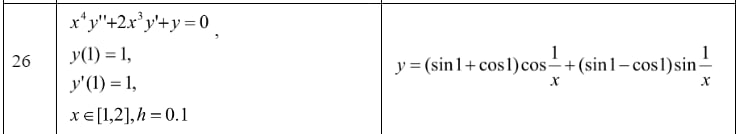
\includegraphics[width=15cm, height=3cm]{img1_1}
\caption{Входные данные}
\end{figure}
% \pagebreak

\subsection{Результаты работы}
\begin{figure}[h!]
\centering
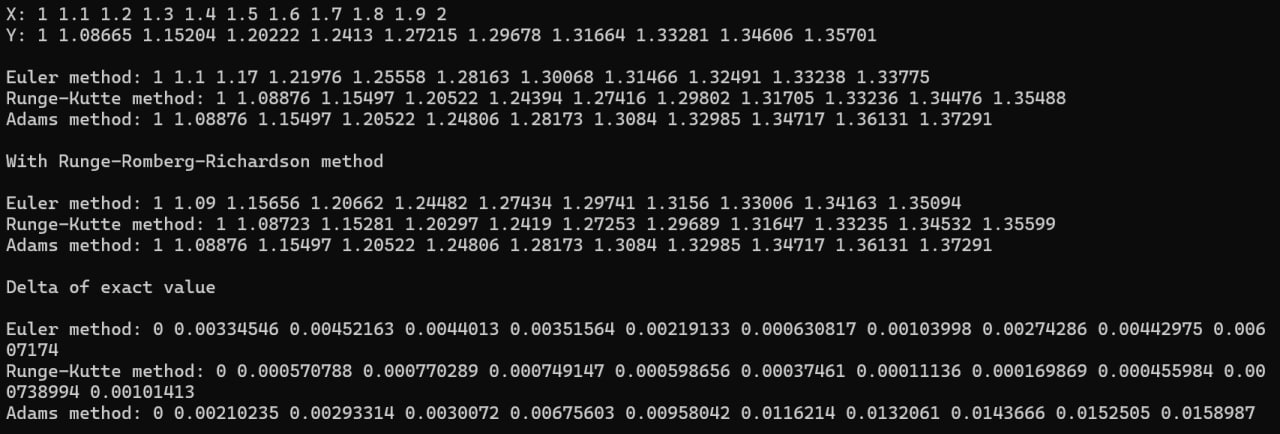
\includegraphics[width=15cm, height=7.5cm]{img1_2}
\caption{Вывод программы в консоли}
\end{figure}

\pagebreak

\subsection{Исходный код}

\lstinputlisting{include/lab4-1.cpp}
\pagebreak

\section* {4.2 Метод стрельбы и конечно-разностный метод}

\subsection{Постановка задачи}
Реализовать метод стрельбы и конечно-разностный метод решения краевой задачи для ОДУ в виде программ. С использованием разработанного программного обеспечения решить краевую задачу для обыкновенного дифференциального уравнения 2-го порядка на указанном отрезке. Оценить погрешность численного решения с использованием метода Рунге – Ромберга и путем сравнения с точным решением. 

{\bfseries Вариант:} 26

\begin{figure}[h!]
\centering
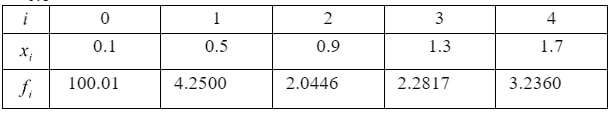
\includegraphics[width=.9\textwidth]{img2_1}
\caption{Входные данные}
\end{figure}
% \pagebreak

\subsection{Результаты работы}
\begin{figure}[h!]
\centering

\includegraphics[width=.9\textwidth]{img2_2}
\caption{Вывод программы в консоли}
\end{figure}

\pagebreak

\subsection{Исходный код}

\lstinputlisting{include/lab4-2.cpp}
